\chapter{Implémentations pour un usage industriel}
\label{chap:erysichtonConception}


Ce chapitre permet de présenter le raisonnement qui a motivé la conception d'un outil de détection automatique de failles par canal auxiliaire de type temporel.

\section{Identification des besoins et spécificités}

Nous avons pu voir grâce aux chapitres précédents que la conception et l'implémentation d'un système sécurisé est un problème difficile. Une première étape est de concevoir des primitives et des protocoles mathématiquement sécurisés. Une seconde étape est de s’assurer que leurs implémentations sont effectivement sécurisées, d'un point de vue : 

\begin{itemize}
    \item mathématique contre des attaques logiques (aspect fonctionnel : le code implémente correctement les bons concepts cryptographiques)
    \item matériel, contre des attaques très bas niveau (les attaques temporelles)
\end{itemize}

Avec l'objectif de concevoir un système sûr, il nous faut donc identifier toutes les tâches à réaliser pour arriver à bout de ce projet. En plus de ce travail de planification, l'identification et l'intégration d'outils déjà implémentés nous permettra d'avancer plus rapidement vers cet objectif.\smallbreak


\subsection*{Point de départ}

En reprenant ces deux étapes, nous identifions les possibilités pour un développeur pour concevoir un système résistant à ces attaques temporelles.\smallbreak

La première étape de conception de primitives cryptologiques et de protocole n'est pas du ressort du développeur. Elle appartient aux cryptologues et aux chercheurs en sécurité mathématique. Ce sont eux qui conçoivent et maintiennent des bibliothèques cryptographiques, des boîtes à outils qui proposent les briques de sécurité nécessaires aux systèmes sécurisés.\medbreak

Plusieurs bibliothèques existent \cite{OpenSSL, BearSSL, polubelova2020haclxn} et remplissent différents objectifs :  rétrocompatiblité, politique temps constant, \etc. Notre choix est à réaliser en fonction des spécificités du produits que nous cherchons à déployer.\medbreak

La seconde étape est à distinguer en deux parties. Cette opération de vérification de la sécurité de l'implémentation peut être réalisée sur le produit fini et sur les bibliothèques employés par le produit. Comme introduit, cette étape a pour objectif la vérification formelle du code du programme et la vérification matérielle au niveau assembleur.\medbreak

Utiliser la bibliothèque \textbf{HACL*} \cite{polubelova2020haclxn, HACL*} permet d'avancer la première étape et la première partie de la seconde étape. Cette bibliothèque a été conçue formellement et vient avec les preuves mathématiques de la sécurité de son implémentation. Comme présenté en \nameref{chap:prelude}, elle est programmée en F*. Le projet permet une exploitation en C et en assembleur \cite{HACL*}.\medbreak

En revanche, la seconde étape de la seconde partie nous demande une vérification au niveau de l'assembleur. Si certaine partie de cette bibliothèque sont codées en assembleur, la majorité du projet reste du F* traduit vers C. Il faut réaliser une analyse. Dans le cadre de cette étude, l'outil d'analyse binaire retenu pour réaliser cette tâche est \textbf{Binsec}. Cet outil est implémenté en Ocaml et il est maintenu par une équipe de chercheurs et d'ingénieurs du CEA-List de Saclay.\medbreak

L'objectif est donc d'analyser HACL* dans son entièreté. Avec cette analyse complète, si elle est correcte, alors les deux étapes de réalisation d'un système sûr seront réalisées. Cela signifie qu'elle sera la première bibliothèque cryptographique formellement sûre et vérifiée résistante aux attaques temporelles.

\subsection*{Objectifs à réaliser}

Sans reprendre les explications du fonctionnement de Binsec, voir \textcolor{red}{"ref vers fonctionement de Binsec"}, l'analyse se réalise sur un fichier binaire à l'aide d'instructions à adjoindre. Avec ce point de départ, nous commençons à construire notre carnet de spécifications.

\textbf{Fichier binaire.} Il faut donc des fichiers binaires à fournir à Binsec. Or comme chacun le sait, plus un binaire est imposant, plus son analyse est difficile. Et comme Binsec emploie l'analyse symbolique, explorer un binaire imposant a un coût de mémoire quadratique sur le parcours des instructions du binaire. L'idéal est donc d'analyser plein de petits fichiers binaires.\smallbreak

\textbf{Analyse complète.} Chaque fonction de HACL* doit être analysée. En poursuivant la condition précédente, nous pouvons essayer de concevoir un binaire par fonction analysée. Nous distribuons ainsi l'analyse et nous parcourons ainsi toute les fonctions présentes dans la bibliothèque.\medbreak

\textbf{Analyse correcte.} En se rappelant comment fonctionnent les optimisations (voir le tableau \ref{tab:compile_option}) il nous faut être attentif avec certaines qui simplifient/modifient le code. Pour éviter des suppressions d'instructions, le fichier nécessite une légère contextualisation avant l'appel de la fonction analysée.

\begin{listing}[!ht]
    \caption{Code d'analyse de la fonction Hacl\_AEAD\_Chacha20Poly1305\_Simd128\_encrypt, testé lors de la prise en main de Binsec et HACL*}
    \label{lst:prise_en_main}
    \begin{minted}[frame=lines,framesep=2mm,baselinestretch=1.2,fontsize=\footnotesize,linenos, gobble=8]{C}
        #include <stdlib.h>

        #include "Hacl_AEAD_Chacha20Poly1305_Simd128.h"

        #define BUF_SIZE 16384
        #define KEY_SIZE 32
        #define NONCE_SIZE 12
        #define AAD_SIZE 12
        #define TAG_SIZE 16

        uint8_t plain[BUF_SIZE];
        uint8_t cipher[BUF_SIZE];
        uint8_t aead_key[KEY_SIZE];
        uint8_t aead_nonce[NONCE_SIZE];
        uint8_t aead_aad[AAD_SIZE];
        uint8_t tag[16];

        int main (int argc, char *argv[])
        {
        Hacl_AEAD_Chacha20Poly1305_Simd128_encrypt
            (cipher, tag, plain, BUF_SIZE, aead_aad, AAD_SIZE, aead_key, aead_nonce);
        exit(0);
        }
    \end{minted}
\end{listing}

De même, comme nos fichiers analysés appartiennent à la bibliothèque extérieur HACL*, l'emploi de l'option \texttt{-static} est nécessaire pour prévenir la mise place de liens vers la bibliothèque partagée dans le fichier binaire. Cette option ne nuit pas à la qualité de l'analyse, elle permet en revanche d'avoir tous les éléments sous la main lorsque nous désassemblons un fichier binaire. Retirer cette option lors de la compilation, c'est s'ajouter des lourdeurs et rallonger le temps requis pour la vérification manuelle d'un fichier.\medbreak

\textbf{Couverture de compilateur.} Les travaux de \citeauthor{schneider2024breakingbadcompilersbreak} \cite{schneider2024breakingbadcompilersbreak} ont clairement mis en évidence que le choix du compilateur est à considérer. Nous allons pouvoir identifier quel compilateur nous permet d'avoir le plus de fichiers binaires sécurisés. Cette analyse nous permet d'identifier les limites de la pratique de la programmation en temps constant.

\textbf{Couverture d'architectures.} x86\_64 et ARM sont les architectures matérielles les plus répandues dans le monde. Étendre l'analyse vers différentes plateformes et observer les différences qui émergent nous permettra d'avancer dans la direction de la conception d'une bibliothèque cryptographique universelle. Nous pouvons aussi étendre cette analyse vers d'autres architectures comme PowerPC ou RiscV.\medbreak


\textbf{Automatisation.} Faire cette analyse sur un fichier binaire, comme le code \ref{lst:prise_en_main}, avec trois axes de complexité (complétude, de la couverture d'architectures et des compilateurs) n'est pas envisageable à la main. Il faut absolument que cette analyse soit automatisée.


\section{Initialisation et tests variés}

Dans le cadre de la programmation sécuritaire, où sont développés les systèmes avec pour objectif d'un accident par siècle (métros automatiques, trains, avions\dots), les projets sont conçus selon le principe du cycle en V. Cette méthode au contraire de la méthode Agile permet de prévoir tous les cas de figure et d'usages, nous permettant de nous épargner les problèmes de correction de bogues.

\begin{figure}[!ht]
    \caption{Cycle en V}
    \label{fig:cycle_en_V}
    \centering
   \begin{tikzpicture}[
        auto,
        mynode/.style={draw, text width=2.5cm, align=center, font=\small},
        myarrow/.style={-Stealth, thick}
    ]

    % Nodes for the V-model
    \node[mynode] (req) {Besoin et exigences};
    \node[mynode, xshift=1cm, yshift=-0.5cm, below of=req] (spec) {Spécification système};
    \node[mynode, xshift=1cm, yshift=-0.5cm, below of=spec] (design) {Conception globale};
    \node[mynode, xshift=1cm, yshift=-0.5cm, below of=design] (detaildesign) {Conception détaillée};
    \node[mynode, xshift=1.3cm, yshift=-0.5cm, below of=detaildesign] (coding) {Codage et implémentation};
    \node[mynode, xshift=2cm, yshift=0.5cm, above of=coding] (unit) {Tests unitaires};
    \node[mynode, xshift=1cm, yshift=0.5cm, above of=unit] (integration) {Tests d'intégration};
    \node[mynode, xshift=1cm, yshift=0.5cm, above of=integration] (system) {Tests système};
    \node[mynode, xshift=1cm, yshift=0.5cm, above of=system] (acceptance) {Tests d'acceptation};
    \node[mynode, above of=acceptance] (maintenance) {Maintenance};

    % Arrows for the V-model
    \draw[myarrow] (req) -- (spec);
    \draw[myarrow] (spec) -- (design);
    \draw[myarrow] (design) -- (detaildesign);
    \draw[myarrow] (detaildesign) -- (coding);
    \draw[myarrow] (coding) -- (unit);
    \draw[myarrow] (unit) -- (integration);
    \draw[myarrow] (integration) -- (system);
    \draw[myarrow] (system) -- (acceptance);
    \draw[myarrow] (acceptance) -- (maintenance);

    % Arrows for the verification and validation
    \draw[myarrow, dashed, opacity=0.5] (unit.west) -- (detaildesign);
    \draw[myarrow, dashed, opacity=0.5] (integration.west) -- (design);
    \draw[myarrow, dashed, opacity=0.5] (system.west) -- (spec);
    \draw[myarrow, dashed, opacity=0.5] (acceptance.west) -- (req);

    % Legend
    \node[draw, opacity=0.5] (legend1) at (10,-2) {};
    \draw[myarrow, dashed, opacity=0.5] (legend1.east) -- ++(1,0);
    \node[anchor=west] at (11,-2) {Vérifications};

    \node[draw] (legend2) at (10,-3) {};
    \draw[myarrow] (legend2.east) -- ++(1,0);
    \node[anchor=west] at (11,-3) {Étapes successives};

    \end{tikzpicture}
\end{figure}
\begin{center}
    \rule{0.75\textwidth}{1pt}
\end{center}

Appliquer cette méthode à l'entièreté de ce projet n'est pas envisageable à cause du coût temporel qui est très élevé. Nous nous concentrons sur la réalisation d'une preuve de concept avec un produit minimal mais opérationnel. Le développement sera concentré sur l'objectif d'automatisation. Le développement d'outils permettant la réalisation des objectifs des couvertures  nécessiteront un futur travail.

\subsection*{Identification des besoins et exigences}

Nous avons déjà conçu notre carnet d'exigences. En revanche nous ne connaissons pas le comportement des outils que nous souhaitons employer. La première opération est donc de s'approprier le fonctionnement de ceux-ci. Le code \ref{lst:prise_en_main} est un exemple de test réalisé dans cette phase du projet.

Binsec est un outil uniquement utilisable au travers d'un terminal. Il s'invoque avec son alias, le binaire à analyser et les options qui seront effectuées :

\begin{listing}[!ht]
    \caption{Commande Binsec basique}
    \label{lst:commande_binsec}
    \begin{minted}{shell}
$ binsec -sse -sse-script $(BINSEC_SCRIPT) -checkct $(BINARY)
    \end{minted}
\end{listing}

L'option \texttt{-sse} permet d'activer l'analyse par exécution symbolique, \texttt{-sse-script} associé à un fichier (ici \texttt{BINSEC\_SCRIPT}) permet d'instruire notre analyse, préciser des stubs\footnote{Terme anglais du lexique de la rétro-ingénierie; module logiciel simulant la présence d'un autre.} et des initialisations. Enfin \texttt{-checkct} active la vérification de la politique temps constant au sein du fichier binaire indiqué par \texttt{BINARY}. Binsec renvoie dans le terminal le résultat de son analyse : [\texttt{secure, unknown, insecure}]. Le second est invoqué lorsque l'analyse est incomplète.\medbreak

Cette phase <<Test et Identification des exigences>> permet de confronter plusieurs fonctions de HACL* et de se familiariser avec le langage d'instructions qu'admet l'option \texttt{-sse-script}. Un tutoriel complet est accessible pour comprendre le fonctionnement l'outil Binsec depuis sa page officielle\footnote{https://binsec.github.io/}.

\begin{listing}[!ht]
    \caption{Instructions permettant de trouver le mot d'un passe d'un binaire exercice}
    \label{lst:exemple_binsec}
    \begin{minted}[frame=lines,framesep=2mm,baselinestretch=1.2,linenos]{bash}
starting from core with
  argv<64> := rsi
  arg1<64> := @[argv + 8, 8]
  size<64> := nondet            # 0 < strlen(argv[1]) < 128
  assume 0 < size < 128
  all_printables<1> := true
  @[arg1, 128] := 0
  for i<64> in 0 to size - 1 do
    @[arg1 + i] := nondet as password
    all_printables := all_printables && " " <= password <= "~"
  end
  assume all_printables
end

replace <puts>, <printf> by
return
end

reach <puts> such that @[rdi, 14] = "Good password!"
then print ascii stream password

cut at <puts> if @[rdi, 17] = "Invalid password!"

halt at <printf>
\end{minted}
\end{listing}

Ce code présenté ici est un exemple d'usage de Binsec et permet de réaliser une attaque sur un binaire issu d'une plateforme d'apprentissage à la sécurité logicielle\footnote{https://crackmes.one/}. L'exercice consiste à retrouver le mot de passe caché d'un binaire. Dans le cadre de notre exercice d'analyse de la politique temps constant, le script \ref{lst:analyse_simple_binsec} est plus simple.\medbreak

Ce script a pour objectif de vérifier les résultats apportés par \cite{schneider2024breakingbadcompilersbreak} concernant une fuite présente sur la fonction <<\textit{FStar\_UInt64\_eq\_mask}>> et d'étendre cette analyse vers d'autres architectures. Dans une première démarche d'automatisation, ce code a été généré automatiquement par un script shell. Nous pouvons voir que l'analyse ne parcourt pas l'entièreté du binaire, seulement 8 sections sont chargées (sur 24). L'analyse commence à l'appel de la fonction \texttt{main} et se termine à la ligne 8 avec une adresse de fin. Cette adresse de fin est produite par le script shell pour attraper la fin de la fonction \texttt{main}. 

\begin{listing}[!ht]
    \caption{Instructions permettant d'analyser le code \ref{lst:Hacl_masking} compilé vers RiscV-32}
    \label{lst:analyse_simple_binsec}
    \begin{minted}[frame=lines,framesep=2mm,baselinestretch=1.2,linenos]{bash}
load sections .plt, .text, .rodata, .data, .got, .got.plt, .bss from file

secret global  r, cin, y, x

starting from <main>

with concrete stack pointer
halt at  0x0000000000000464
explore all

\end{minted}
\end{listing}


Ce modèle, qui nous servira de base pour la suite du développement, a permis une analyse rapide entre différents compilateurs et différentes architectures.

\subsection*{Application et observation entre architectures et compilateurs}


\begin{figure}[!ht]
    \caption{Tableau de résultats d'analyse Binsec pour architecture ARMv7 et ARMv8}
    \label{tab:resultats_arm}
    \begin{center}    
        \begin{tabular}{|c|c|c|c|c|c|}
            \hline
            \rowcolor{blue!10}
            \cellcolor{inria-2024-gris-bleu!20}\textbf{opt}\textbackslash\textbf{fonction analysée} & \multicolumn{5}{c|}{\textbf{cmovznz4}} \\
            \hline
            \rowcolor{blue!30}
            \textbf{Clang+LLVM} & \textbf{14.0.6} & \textbf{15.0.6} & \textbf{16.0.4} & \textbf{17.0.6} & \textbf{18.1.8} \\
            \hline
            \rowcolor{orange!30!red!50}
            \textbf{-O0} & \cellcolor{green!60}\checkmark & \cellcolor{green!60}\checkmark & \cellcolor{green!60}\checkmark  & \cellcolor{green!60}\checkmark  & \cellcolor{green!60}\checkmark  \\
            \hline
            \rowcolor{orange!30!red!50}
            \textbf{-O1} & \cellcolor{green!60}\checkmark & \cellcolor{green!60}\checkmark & \cellcolor{green!60}\checkmark  & \cellcolor{green!60}\checkmark  & \cellcolor{green!60}\checkmark  \\
            \hline
            \rowcolor{orange!30!red!50}
            \textbf{-O2} & \cellcolor{green!60}\checkmark & \cellcolor{green!60}\checkmark & \cellcolor{green!60}\checkmark  & \cellcolor{green!60}\checkmark  & \cellcolor{green!60}\checkmark  \\
            \hline
            \rowcolor{orange!30!red!50}
            \textbf{-O3} & \cellcolor{green!60}\checkmark & \cellcolor{green!60}\checkmark  & \cellcolor{green!60}\checkmark  & \cellcolor{green!60}\checkmark  & \cellcolor{green!60}\checkmark  \\
            \hline
            \rowcolor{orange!30!red!50}
            \textbf{-Os} & \cellcolor{green!60}\checkmark  & \cellcolor{green!60}\checkmark  & \cellcolor{green!60}\checkmark  & \cellcolor{green!60}\checkmark  & \cellcolor{green!60}\checkmark  \\
            \hline
            \rowcolor{orange!30!red!50}
            \textbf{-Oz} & \cellcolor{green!60}\checkmark  & \cellcolor{green!60}\checkmark  &  \cellcolor{green!60}\checkmark  &  \cellcolor{green!60}\checkmark  &  \cellcolor{green!60}\checkmark \\
            \hline
        \end{tabular}   
    \end{center}
    \raggedleft
    \small{
    \checkmark : \textit{binary secure}
    }
\end{figure}

Nous comprenons, à la lecture du tableau \ref{tab:resultats_arm}, que la politique temps constant est considérée respectée par Binsec sur les versions testées ainsi que pour les différentes options de compilation. Ce résultat est encourageant pour la suite du projet.\medbreak

\begin{figure}[!htb]
    \caption{Tableau de résultats d'analyse Binsec pour architecture Risc-V}
    \label{tab:resultats_riscv}
    \begin{center}

    \begin{tabular}{|c|cc|cc|}
        \hline
        \rowcolor{blue!10}
        \cellcolor{inria-2024-gris-bleu!20}\textbf{opt}\textbackslash\textbf{fonction analysée} & \multicolumn{2}{c|}{\textbf{cmovznz4} - 64 bits} & \multicolumn{2}{c|}{\textbf{cmovznz4} - 32 bits} \\
        \hline
        \rowcolor{blue!30}
        \textbf{Compilateur et architecture} & gcc 15.1.0 & clang 19.1.7 & gcc 15.1.0& clang 19.1.7 \\
        \hline
        \rowcolor{orange!30!red!50}
        \textbf{-O0} &  \cellcolor{orange!60}\textasciitilde  & \cellcolor{red!60}$\times$ & \cellcolor{orange!60}\textasciitilde & \cellcolor{red!60}$\times$ \\
        \hline
        \rowcolor{orange!30!red!50}
        \textbf{-O1} &  \cellcolor{green!60}\checkmark & \cellcolor{red!60}$\times$ & \cellcolor{green!60}\checkmark & \cellcolor{red!60}$\times$ \\
        \hline
        \rowcolor{orange!30!red!50}
        \textbf{-O2} &  \cellcolor{green!60}\checkmark & \cellcolor{red!60}$\times$ & \cellcolor{green!60}\checkmark & \cellcolor{red!60}$\times$ \\
        \hline
        \rowcolor{orange!30!red!50}
        \textbf{-O3} &  \cellcolor{green!60}\checkmark & \cellcolor{red!60}$\times$ & \cellcolor{green!60}\checkmark & \cellcolor{red!60}$\times$ \\
        \hline
        \rowcolor{orange!30!red!50}
        \textbf{-Os} &  \cellcolor{green!60}\checkmark & \cellcolor{red!60}$\times$ & \cellcolor{green!60}\checkmark & \cellcolor{red!60}$\times$ \\
        \hline
        \rowcolor{orange!30!red!50}
        \textbf{-Oz} &  \cellcolor{green!60}\checkmark & \cellcolor{red!60}$\times$ & \cellcolor{green!60}\checkmark & \cellcolor{red!60}$\times$ \\
        \hline
    \end{tabular}
    \end{center}
    \raggedleft
     \small{
        \checkmark : \textit{binary secure} ;
        \textasciitilde : \textit{binary unknown} ;
        $\times$ : \textit{binary insecure}
    }
\end{figure}

Les résultats dans le tableau \ref{tab:resultats_riscv} sont indéniables : la version 19.1.7 de clang rend le code source perméable à des attaques temporelles.\medbreak

\begin{CitationBox}{Identification de défaut}
    Pour construire le tableau \ref{tab:resultats_riscv}, plusieurs alertes se sont levées et ont permis de mettre en évidence un bug présent dans Binsec. Cette erreur dans l'analyse symbolique provoquait l'arrêt de l'exploration par explosion de l'usage de la mémoire. Les registres \texttt{ld} (\textit{load}) et \texttt{sd} (\textit{store}) étaient mal gérés. En particulier l'opérande \texttt{ld}, simulé par un tableau, n'était jamais vidé. Cette découverte a amené un correctif et une amélioration de Binsec. De par l'envergure de ce projet, il est possible que d'autres erreurs dues à Binsec soient découvertes. L'exploration de nombreuses et nouvelles ISA\footnote{Acronyme anglais pour Architecture de Jeu d'Instruction, désigne l'ensemble des instructions assembleur associées à une architecture.}, surtout avec Risc-V qui est encore en développement et perfectionnement, permet de renforcer cet outil plus efficacement et rapidement que par la conception de tests manuels.\medbreak
\end{CitationBox}
    
    


En explorant plus en avant le code binaire, nous découvrons que ces erreurs sont dues à l'opérande \texttt{beqz}\footnote{Effectue un branchement si la valeur du registre consulté est zéro. Cette opérande est propre à Risc-V.}. L'ISA de Risc-V n'a pas à sa disposition un opérande comme \texttt{cmov} en X86\_64 ou ARM. Donc l'application d'optimisation de compilation force l'usage de cette opérande qui n'est pas en temps constant. L'optimisation qui réalise ce changement se nomme <<\textit{InstCombinePass}>>.\medbreak

Nous observons ici une manifestation indéniable des précédents résultats proposés par d'autres travaux de recherche. Une solution serait de modifier l'ISA pour permettre cette opération d'être en temps constant. Celle qui a été retenue, c'est d'employer un \texttt{pragma}, ici \texttt{\# pragma clang optimise <off/on>}. Cette instruction, donnée dans le code source, indique au compilateur de désactiver ses optimisations pour le code contenu entre les deux balises \texttt{off,on}. Cette solution entraîne des pertes de performance et des ralentissements quant au temps de compilation et à l'usage des ressources. Il est donc préférable de l'utiliser avec parcimonie.\medbreak

Après avoir ciblé notre besoin, les exigences associées et effectué des tests pour comprendre le processus à automatiser, nous pouvons synthétiser la démarche avec la figure \ref{fig:compilation_simple} : depuis HACL*, nous extrayons une fonction qui sera testé, nous fabriquons le fichier de test en C; nous identifions les paramètres secrets et nous concevons le script adéquat pour Binsec; nous compilons le fichier C à notre guise et nous terminons par l'analyse Binsec.

\begin{figure}[!ht]
    \caption{Flot de travail de l'outil d'analyse à concevoir}
    \label{fig:compilation_simple}
    \centering
    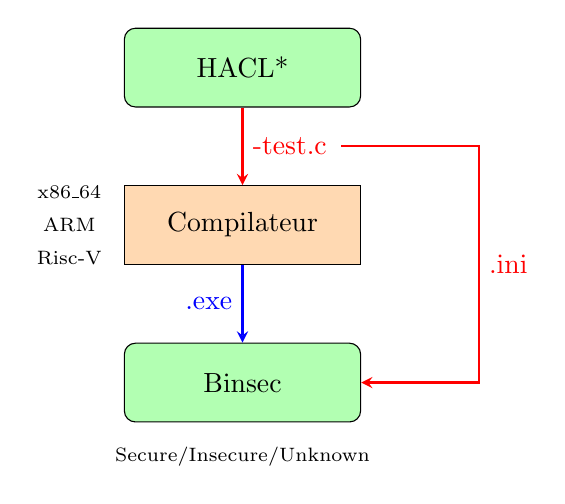
\begin{tikzpicture}[node distance=2cm]

    % Styles des noeuds
    \tikzstyle{startstop} = [rectangle, rounded corners, minimum width=3cm, minimum height=1cm,text centered, draw=black, fill=green!30]
    \tikzstyle{process} = [rectangle, minimum width=3cm, minimum height=1cm, text centered, draw=black, fill=orange!30]
    \tikzstyle{intermediate} = [circle, minimum size=0.5cm, text centered, draw=white, fill=white]
    \tikzstyle{arrow} = [thick,->,>=stealth]
    
    % Noeuds
    \node (hacl) [startstop] {HACL*};
    \node (inter) [intermediate, below of=hacl,xshift=1cm, yshift=1cm] {};
    \node (compilateur) [process, below of=hacl] {Compilateur};
    \node (binsec) [startstop, below of=compilateur] {Binsec};
    
    % Flèches
    \draw [arrow, red] (hacl) -- node[anchor=west] {-test.c} (compilateur);
    \draw [arrow, red] (inter) -- ++(2,0) |- node[anchor=west, pos=0.25] {.ini} (binsec);
    \draw [arrow, blue] (compilateur) -- node[anchor=east] {.exe} (binsec);
    
    % Annotations
    \node[align=center, left of=compilateur, xshift=-0.2cm] {\scriptsize x86\_64\\ \scriptsize ARM\\ \scriptsize Risc-V};
    \node[align=center, below of=binsec, yshift=30pt] {\scriptsize Secure/Insecure/Unknown};
    
    \end{tikzpicture}

\end{figure}

\vfill
\textit{Nous allons maintenant nous pencher sur le procédé de conception de notre outil de détection automatique de failles temporelles.}





